% !TEX TS-program = pdflatex
% !TEX encoding = UTF-8 Unicode

% This is a simple template for a LaTeX document using the "article" class.
% See "book", "report", "letter" for other types of document.

\documentclass[11pt]{article} % use larger type; default would be 10pt

\usepackage[utf8]{inputenc} % set input encoding (not needed with XeLaTeX)

%%% Examples of Article customizations
% These packages are optional, depending whether you want the features they provide.
% See the LaTeX Companion or other references for full information.

%%% PAGE DIMENSIONS
\usepackage{geometry} % to change the page dimensions
\geometry{a4paper} % or letterpaper (US) or a5paper or....
% \geometry{margin=2in} % for example, change the margins to 2 inches all round
% \geometry{landscape} % set up the page for landscape
%   read geometry.pdf for detailed page layout information

\usepackage{graphicx} % support the \includegraphics command and options
\usepackage{topcapt}

% \usepackage[parfill]{parskip} % Activate to begin paragraphs with an empty line rather than an indent

%%% PACKAGES
\usepackage{booktabs} % for much better looking tables
\usepackage{array} % for better arrays (eg matrices) in maths
\usepackage{paralist} % very flexible & customisable lists (eg. enumerate/itemize, etc.)
\usepackage{verbatim} % adds environment for commenting out blocks of text & for better verbatim
\usepackage{subfig} % make it possible to include more than one captioned figure/table in a single float
% These packages are all incorporated in the memoir class to one degree or another...

%%% HEADERS & FOOTERS
\usepackage{fancyhdr} % This should be set AFTER setting up the page geometry
\pagestyle{fancy} % options: empty , plain , fancy
\renewcommand{\headrulewidth}{0pt} % customise the layout...
\lhead{}\chead{}\rhead{}
\lfoot{}\cfoot{\thepage}\rfoot{}

%%% SECTION TITLE APPEARANCE
\usepackage{sectsty}
\allsectionsfont{\sffamily\mdseries\upshape} % (See the fntguide.pdf for font help)
% (This matches ConTeXt defaults)

%%%% ToC (table of contents) APPEARANCE
%\usepackage[nottoc,notlof,notlot]{tocbibind} % Put the bibliography in the ToC
%\usepackage[titles,subfigure]{tocloft} % Alter the style of the Table of Contents
%\renewcommand{\cftsecfont}{\rmfamily\mdseries\upshape}
%\renewcommand{\cftsecpagefont}{\rmfamily\mdseries\upshape} % No bold!

%%% END Article customizations

%%% The "real" document content comes below...

\title{Differential gene expression in males vs females for head and neck squamous cancers (HNSC)}
\author{Czuee Morey}
%\date{} % Activate to display a given date or no date (if empty),
         % otherwise the current date is printed 

\begin{document}
\maketitle

The gene expression data for HNSC was taken from the Cancer genome atlas study \cite{nature}. The data contained 566 samples for RNA-seq from males and females. In some cases, normal samples from the same individual were also present. The data was treated suitably for analysis. In part 1, the normal tissues were removed and only tumor samples were considered. In part 2, the samples for which both tumor and normal tissue are present were considered. The log of gene expression(+1) was considered for all cases, and the expression was centered around the mean in some cases.

\begin{figure}[htbp]
\centering
\subfloat{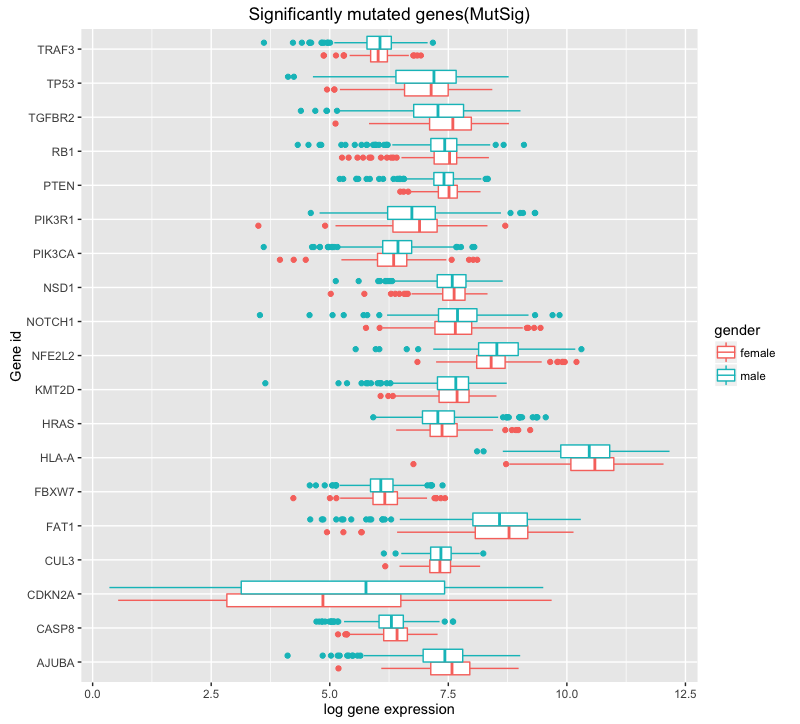
\includegraphics[width=0.5\textwidth]{Plots/Expression_mutsig_genes.png}}
\subfloat{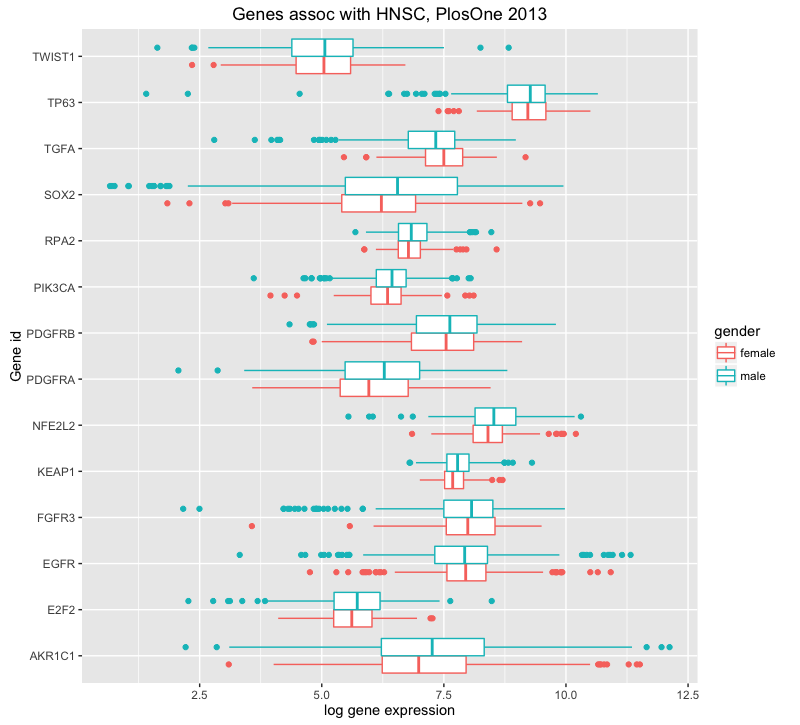
\includegraphics[width=0.5\textwidth]{Plots/Exp_HNSC-genes_Pone.png}}
\caption{Significantly mutated genes \cite{nature} and genes associated with HNSC \cite{pone} do not show differential expression between males and females.}
\label{mutsig}
\end{figure}

\section{Gene expression in tumors}

\subsection{Selecting genes with highest variability}

The genes were filtered to select only genes that would have the highest variance in their gene expression and are more likely to have differential expression between males and females. The genes were sorted by the standard deviation (SD) of gene expression over all samples (figure~\ref{sd-plot}). The top 2,000 genes were used for further analysis.

\begin{figure}[htbp]
\centering
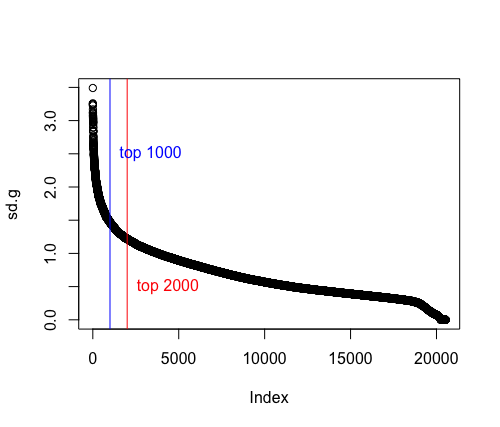
\includegraphics[width=0.5\textwidth]{Plots/SD-plot_top1k2k.png}
\caption{Plot for Standard deviation of gene expression ordered from highest to lowest. The vertical lines indicate the position for first 1000 and 2000 genes that were selected for further study.}
\label{sd-plot}
\end{figure}

\subsection{Genes with significant difference in means between males and females}

in ordert o find the genes that are different in males and females, the mean of the distrubution in the two sexes were compared. There were 21 genes which had a significant difference in their means  (figure~\ref{diff-mean}).

\begin{figure}[htb]
\centering
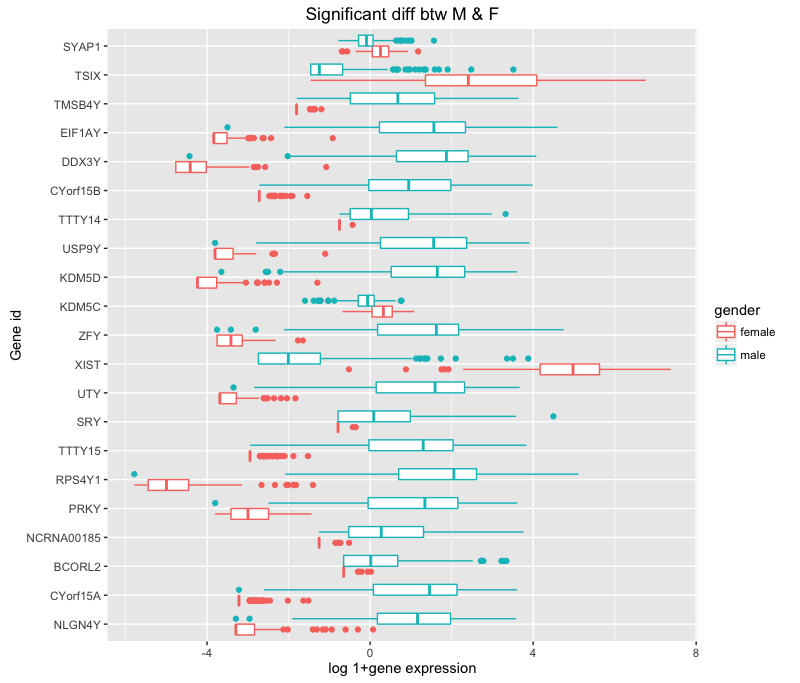
\includegraphics[width=0.6\textwidth]{Plots/Signif21_genenames_boxplot.png}
\caption{The genes that have a difference between their means in males and females greater than the SD of the entire distribution were selected. This analysis resulted in 21 genes.}
\label{diff-mean}
\end{figure}

\begin{table}[htb]
\small
   \centering
   \caption{The genes that have a difference between their means in males and females greater than the SD of the entire distribution were selected. 19 descriptions - NCRNA00185 and TTTY14 are the same gene. Also CYorf15A and B have the same description (TXLNGY). All the genes are X and Y linked only.} % requires the topcapt package
   \begin{tabular}{p{1.5cm} p{10cm} p{2.5cm}} % Column formatting, @{} suppresses leading/trailing space
   \toprule
Approved Symbol & Approved Name & Chromosome \\
\midrule
DDX3Y & DEAD-box helicase 3, Y-linked & Yq11 \\
EIF1AY & eukaryotic translation initiation factor 1A, Y-linked & Yq11.223 \\
KDM5C & lysine demethylase 5C & Xp11.22-p11.21 \\
KDM5D & lysine demethylase 5D & Yq11 \\
NLGN4Y & neuroligin 4, Y-linked & Yq11.221 \\
PRKY & protein kinase, Y-linked, pseudogene & Yp11.2 \\
RPS4Y1 & ribosomal protein S4, Y-linked 1 & Yp11.3 \\
SRY & sex determining region Y & Yp11.3 \\
SYAP1 & synapse associated protein 1 & Xp22.31 \\
TMSB4Y & thymosin beta 4, Y-linked & Yq11.221 \\
TSIX & TSIX transcript, XIST antisense RNA & Xq13.2 \\
TTTY14 & testis-specific transcript, Y-linked 14 (non-protein coding) & Yq11.222 \\
TTTY15 & testis-specific transcript, Y-linked 15 (non-protein coding) & Yq11.1 \\
USP9Y & ubiquitin specific peptidase 9, Y-linked & Yq11.2 \\
UTY & ubiquitously transcribed tetratricopeptide repeat containing, Y-linked & Yq11.221 \\
XIST & X inactive specific transcript (non-protein coding) & Xq13.2 \\
ZFY & zinc finger protein, Y-linked & Yp11.3 \\
BCORP1 & BCL6 corepressor pseudogene 1 & Yq11.222 \\
TXLNGY & taxilin gamma pseudogene, Y-linked & Yq11.222 \\
\bottomrule
   \end{tabular}
   \label{signif1}
\end{table}

Table~\ref{signif1} lists the description and location of these genes. All the genes identified were X or Y linked genes, which obviously have differential expression in males and females. Hence, in the next step, I considered the gene expression difference between tumor and normal samples from the same individual to avoid identifying obvious differences between males and females.

\section{Gene expression difference in tumor minus normal}

Out of the 566 samples, only few samples had tumor and normal tissue data from the same patient and were extracted. The tumor and normal tissue data was present for 14 females and 29 males. In this part, the number fo genes to be considered for analysis was identified as 10,000 genes with highest variance on the basis of a QQ-plot of the SD values.

The data was processed so that the $(tumor - normal)$ values were calculated for each patient. This gave a data frame of (T-N) values for 10,000 gene columns and patient rows. 

\begin{figure}[htbp]
\centering
\subfloat[t-test]{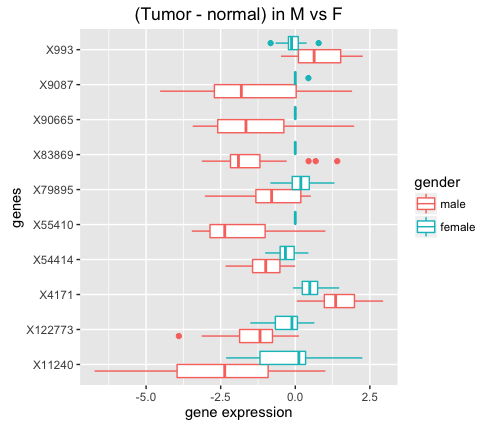
\includegraphics[width=0.4\textwidth]{Plots/Tum-Norm_diff_MvsF_q01.png}}
\subfloat[Wilcoxon test]{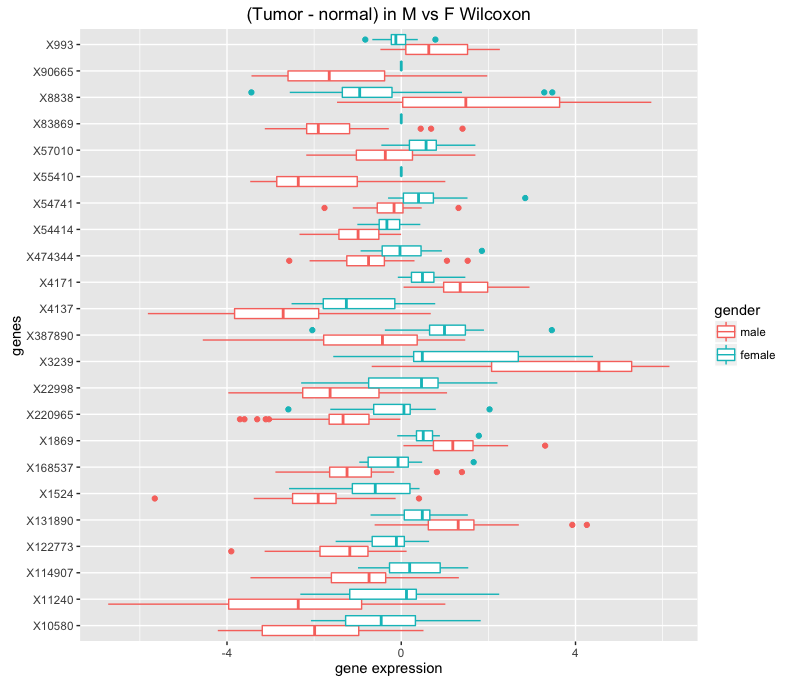
\includegraphics[width=0.6\textwidth]{Plots/MvsF_T-N_Wilcox23.png}}
\caption{Significant genes identified through statistical tests (a) t-test with q-value $<$ 0.1 and (b) Wilcoxin test with P-value $<$ 0.001.}
\label{signif-test}
\end{figure}

The t-test statistic was calculated as a function of gender for each gene. The p-values calculated for each gene were adjusted using the q-value package and p.adjust packages. The Wilcoxon test was also performed and the p-values were used to identify the significant genes. The q-values did not give any significant genes eevn at q $<$ 0.1 with this test. The different methods picked up similar genes. Figure~\ref{signif-test} shows the genes identified through the t-test and Wilcoxin test. The significant genes identified through the t-test are listed in table~\ref{signif2}.

\begin{table}[htb]
\small
   \centering
   \caption{Significant genes identified through the t-test with q-value $<$ 0.1. The Y-linked genes can be considered as false positives.} % requires the topcapt package
   \begin{tabular}{p{1.5cm} p{10cm} p{2.5cm}} % Column formatting, @{} suppresses leading/trailing space
   \toprule
Approved Symbol & Approved Name & Chromosome \\
\midrule
ATP8B4 & ATPase phospholipid transporting 8B4 (putative) & 15q21.2 \\
CDC25A & cell division cycle 25A & 3p21 \\
KLHDC1 & kelch domain containing 1 & 14q21.3 \\
MCM2 & minichromosome maintenance complex component 2 & 3q21 \\
PADI2 & peptidyl arginine deiminase 2 & 1p35.2-p35.1 \\
SIAE & sialic acid acetylesterase & 11q24 \\
TBL1Y & transducin (beta)-like 1, Y-linked & Yp11.2 \\
TMSB4Y & thymosin beta 4, Y-linked & Yq11.221 \\
TTTY14 & testis-specific transcript, Y-linked 14 (non-protein coding) & Yq11.222 \\
\bottomrule
   \end{tabular}
   \label{signif2}
\end{table}
\begin{thebibliography}{9}


\bibitem{nature} 
Network, T. C. G. A. (2015)
\textit{Comprehensive genomic characterization of head and neck squamous cell carcinomas}. 
Nature 517, 576–582.

\bibitem{pone}
Vonn Walter et al (2013)
\textit{Molecular Subtypes in Head and Neck Cancer Exhibit
Distinct Patterns of Chromosomal Gain and Loss of
Canonical Cancer Genes}
Plos One 8(2), e56823.

\end{thebibliography}
\end{document}
